\documentclass[tcc]{subfiles}

\begin{document}

\chapter{Materials and methods}
\label{ch:methods}

\section{The engine} \index{engine} \index{JetsMunt VT80}

The engine for which the \gls{FADEC} will be developed is the JetsMunt VT80.
This engine was developed for hobby use in airplane models and comes with an \gls{ECU} installed from factory, which will not be used for this work.
It is a single spool jet engine, with a single stage centrifugal compressor 
 and also single stage axial turbine, as seen in \cref{fig:engine}. 
It runs on aviation kerosene pre-mixed with oil.%
\footnote{it can use either two-stroke automotive oil at 3\% 
    or turbine oil at 5\%. Check the manual 
    \cite{engine-manual} for details}
The specifications provided by the manufacturer are in \cref{tbl:engine_specs}.
\textcite{bolsoni} estimates the compressor pressure ratio 
to be around 2.2 based on similar engines.

\begin{figure}[p]
    \centering
    \caption{JetsMunt VT-80 jet engine}
    \label{fig:engine}
    \begin{subfigure}{\textwidth}
        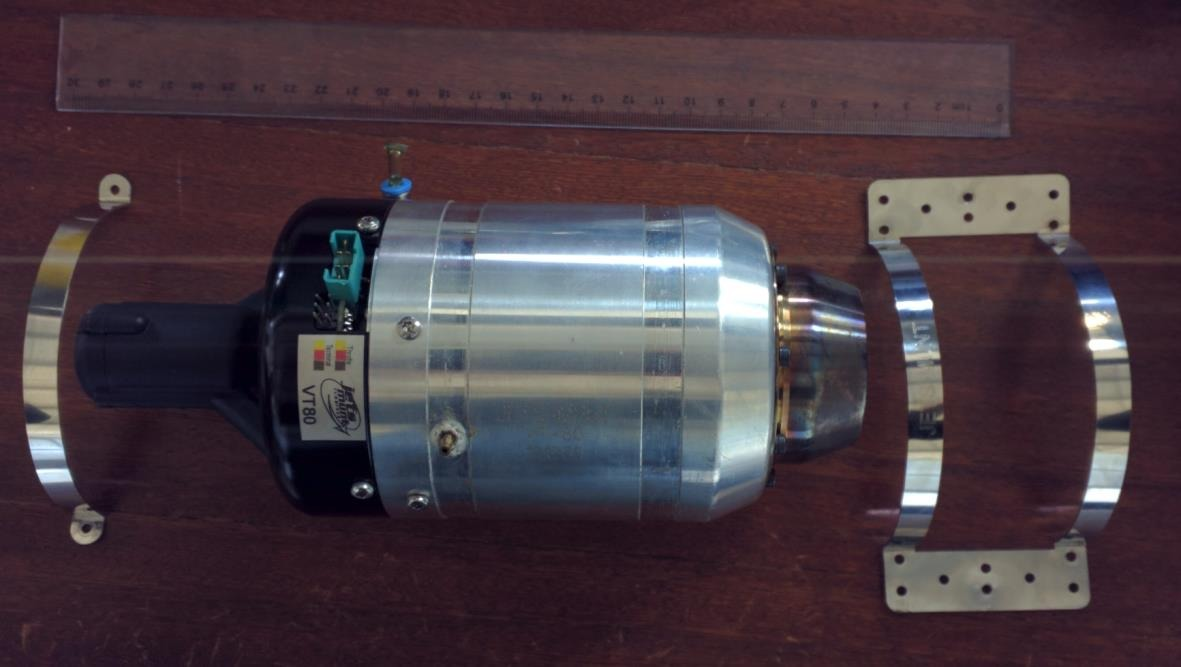
\includegraphics[width=\textwidth]{fig/JetsMuntVT-80.jpg}
        \caption{Picture with a 30cm ruler for scale}
        \label{fig:engine!visible}
    \end{subfigure}
    \begin{subfigure}{\textwidth}
        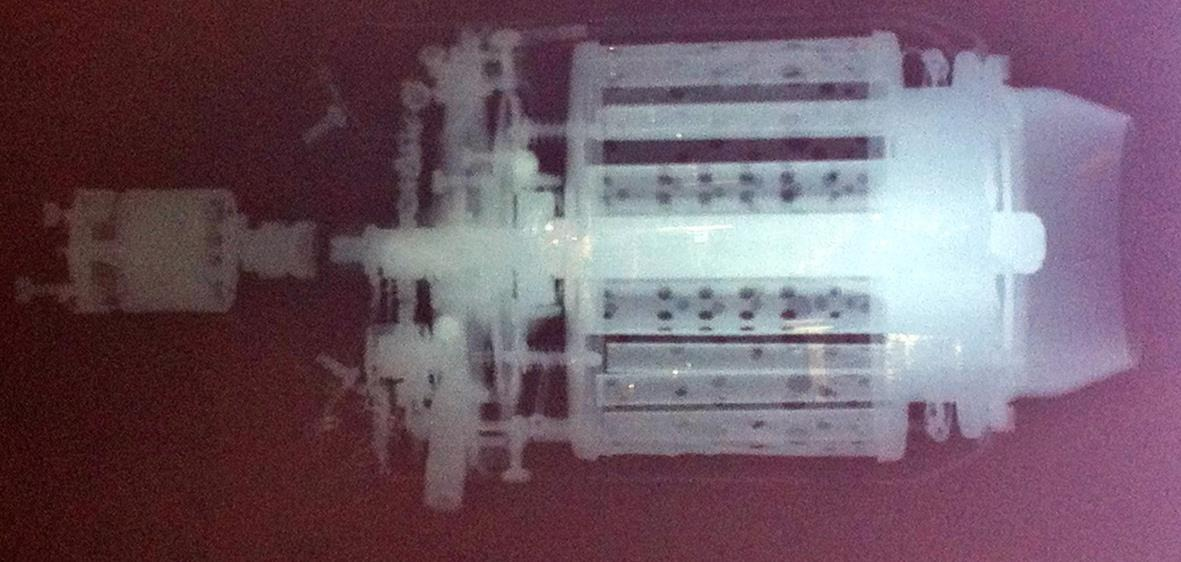
\includegraphics[width=\textwidth]{fig/JetsMuntVT-80X-ray.jpg}
        \caption{X-ray picture}
        \label{fig:engine!x-ray}
    \end{subfigure}
    \source{\cite{bolsoni}}
\end{figure}

\begin{table}
    \centering
    \caption{VT80 Specifications}
    \label{tbl:engine_specs}
    \begin{tabular}{lr@{$\,$}l}
        \toprule
        Diameter (external)                & 90 & mm \\
        Length                             & 240 & mm \\
        Weight (bare)                      & 950 & g \\
        Weight (with accessories)          & 1075 & g \\
        Nominal thrust @ 15C and sea level & 80 & N \\
        Idle thrust                        & 4 & N \\
        Max rpm                            & 150 000 & rpm \\
        Idle rpm                           & 45 000  & rpm \\
        Heat soak rpm                      & 12 000  & rpm \\
        \acs{EGT} @ max rpm                & 600$\pm$50 & \si{\celsius} \\
        Fuel consumption @ max rpm         & 0.29 & L/min \\
        Fuel/oil                   &\multicolumn{2}{l}{Kerosene + 4\% oil} \\
        \bottomrule
    \end{tabular}
    \source{\cite{engine-manual}}
\end{table}

\section{The instrumentation}
The engine was instrumented to provide measurements of the following:
\begin{compactitem}
    \item Ambient pressure
    \item Ambient temperature
    \item Ambient relative humidity
    \item Fuel flow
    \item Air mass flow
    \item Static pressure at compressor exit
    \item Temperature at compressor exit
    \item Temperature at turbine entry
    \item Pressure at turbine exit
    \item Temperature at turbine exit
    \item \gls{EGT}
    \item Shaft rotational speed
    \item Thrust
\end{compactitem}

All pressures are measured by pressure transducers, and temperatures by type K thermocouples. 
Air mass flow is measured through an specially designed admission nozzle. 
Thrust is measured from a load cell installed in the engine mounts.
For a specification of each sensor used, refer to \cref{app:instrumentation}.

All sensors are read though an acquisition card 
model DAQ USB-6009 manufactured by National Instruments 
\cite{acquisition card}.
Every signal was amplified up to this board's operational range (-10V to 10V). 
The data acquired is then processed by a program developed in-house.%
\footnote{this program is available at \todo{put program on github}}

\section{The test bench}

The test bench used for this project was designed and built by Frederico Bolsoni at the \gls{ALFALAB}.
It was made so that its weight is at least ten times the engine thrust 
 and its natural frequencies are separated from those of the engine \cite{bolsoni}.
The test bench is shown in \cref{fig:test_bench}.

\begin{figure}[p]
    \centering
    \caption{Test bench}
    \label{fig:test_bench}
    \begin{subfigure}{.49\textwidth}
        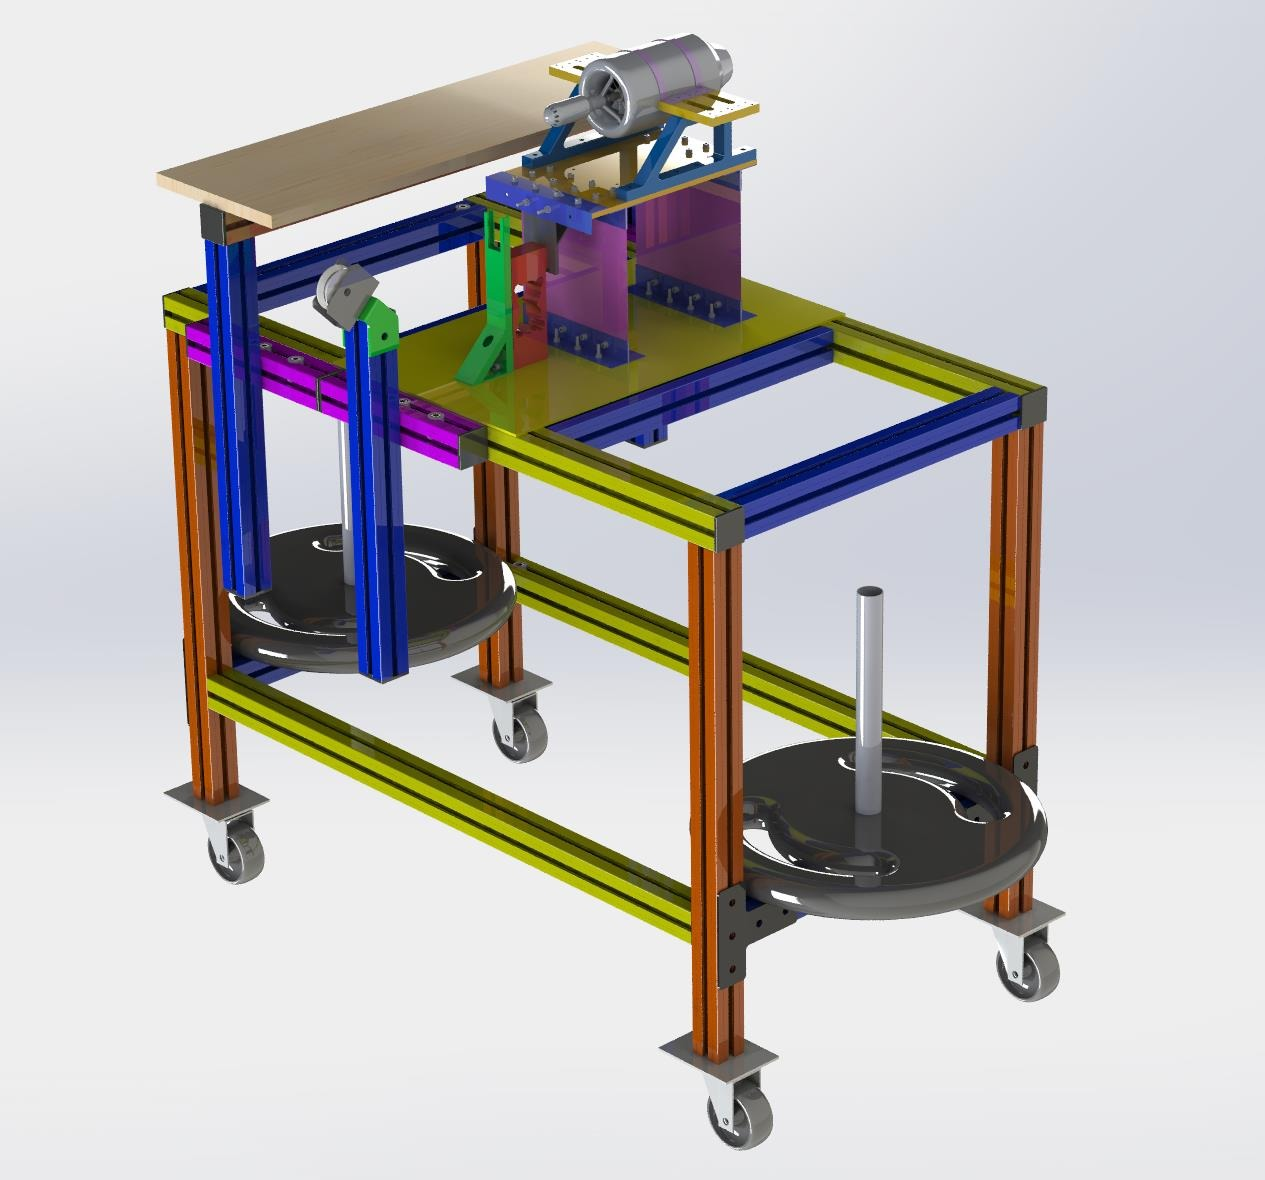
\includegraphics[width=.9\textwidth]{fig/test_bench_rendering.jpg}
        \caption{\acs{CAD} rendering}
        \label{fig:test_bench!rendering}
    \end{subfigure}
    \begin{subfigure}{.49\textwidth}
        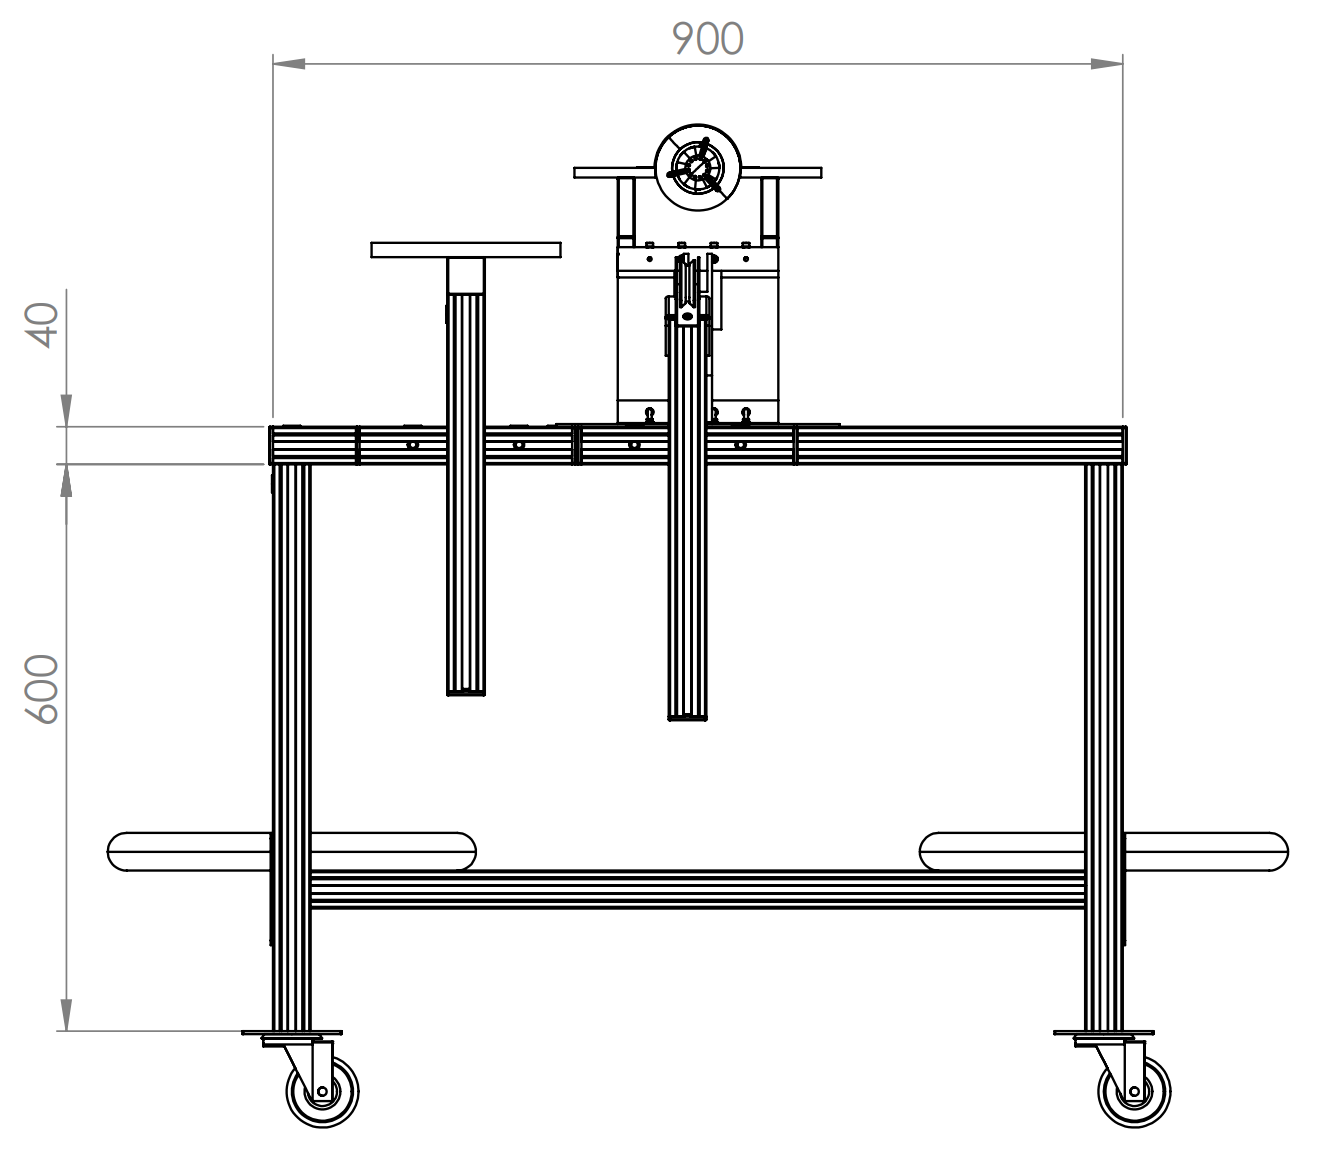
\includegraphics[width=.9\textwidth]{fig/test_bench_drawing.png}
        \caption{Blueprint (dimensions in mm)}
        \label{fig:test_bench!blueprint}
    \end{subfigure}

    \begin{subfigure}{.49\textwidth}
        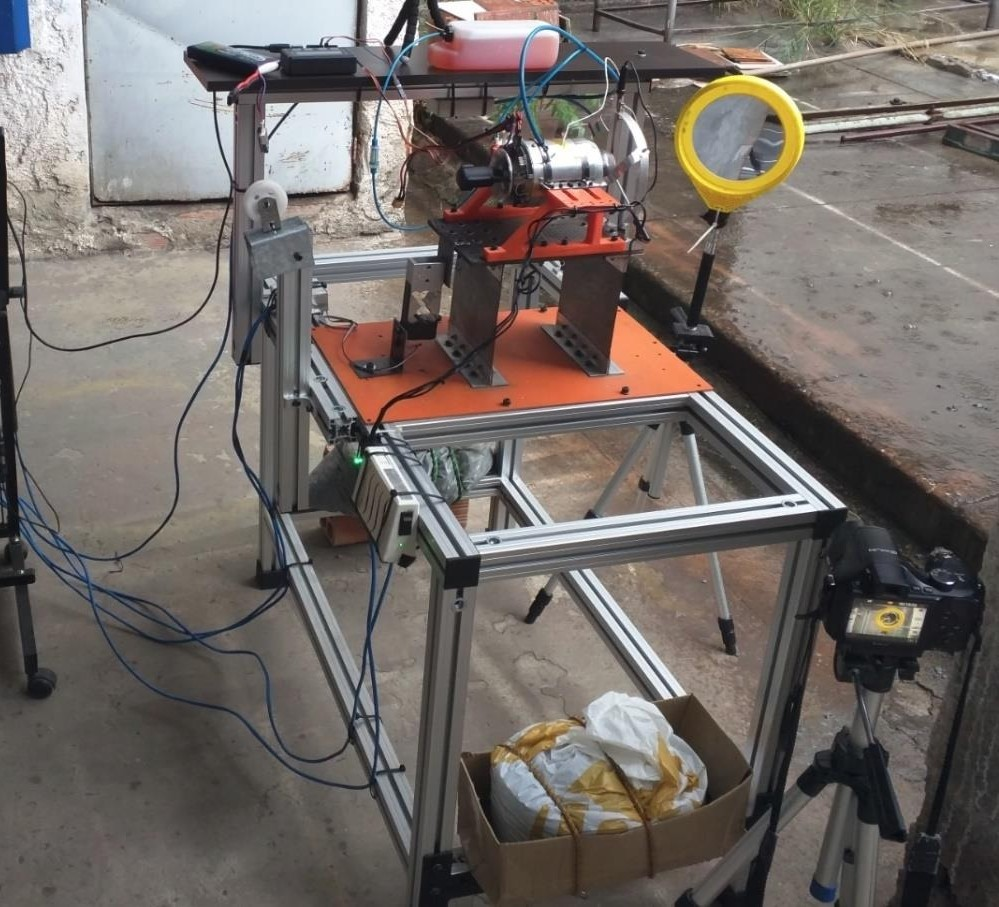
\includegraphics[width=.9\textwidth]{fig/engine_in_bench3.jpg}
        \caption{Picture with engine installed}
        \label{fig:test_bench!picture}
    \end{subfigure}
    \begin{subfigure}{.49\textwidth}
        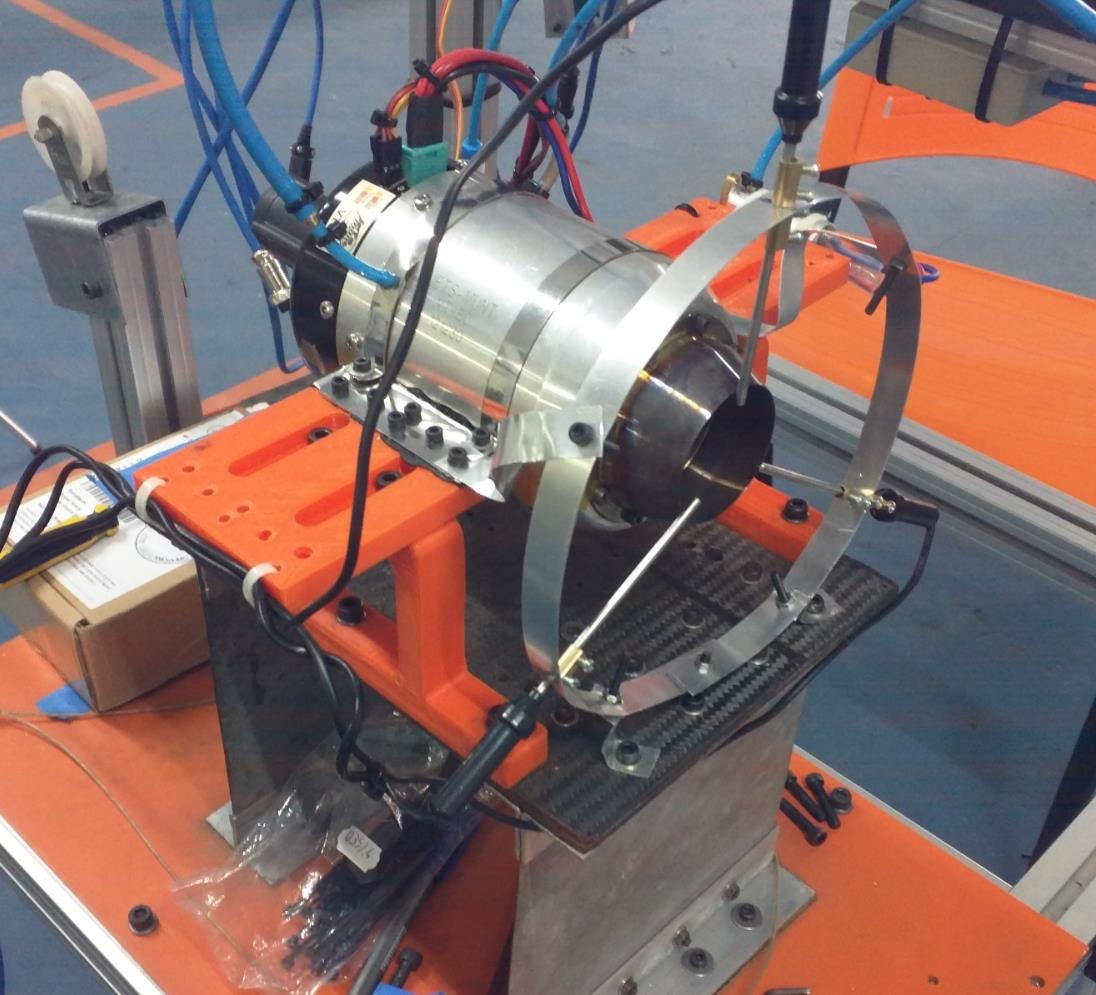
\includegraphics[width=.9\textwidth]{fig/engine_in_bench.jpg}
        \caption{Close up picture with engine installed}
        \label{fig:engine!closeup}
    \end{subfigure}
    \source{\cite{bolsoni}}
\end{figure}
\end{document}
